\addcontentsline{toc}{chapter}{Обзор и анализ робототехнических систем, условия их применения}
\textbf{\underline{В первой главе}} представлены обзор и анализ областей, которые необходимы для решения поставленных научных задач.

Была проведена классификация машин, использующих ноги в качестве движителя. Изучив данный класс машин, были осмыслены габаритные и структурные особенности этих роботов. Для решения задачи определения геометрических и физико-механических свойств пройденной поверхности были изучены типы препятствий и размеры. Задача определения геометрических свойств объекта является частью Mapping из класса методов Simultaneous Localization and Mapping (SLAM). Была выявлена необходимость разработки модифицированного метода 2D триангуляции Делоне для вогнутых оболочек. Были рассмотрены различные алгоритмы и средства определения физико-механических свойств поверхности. Сделан вывод о необходимости использования датчика силы, установленного на ногу робота, а также собирать дополнительные данные об угловой скорости и моменте на моторе.

На основе проведенного анализа, разработана концепция робота \pic{fig:diag_system.png}. Оранжевым цветом выделены компоненты системы, которые представляют собой предмет исследования в рамках диссертационной работы. Голубым цветом выделены блоки, которые были использованы в работе как стандартные средства, без каких-либо существенных доработок.
\begin{figure}[h]
    \centering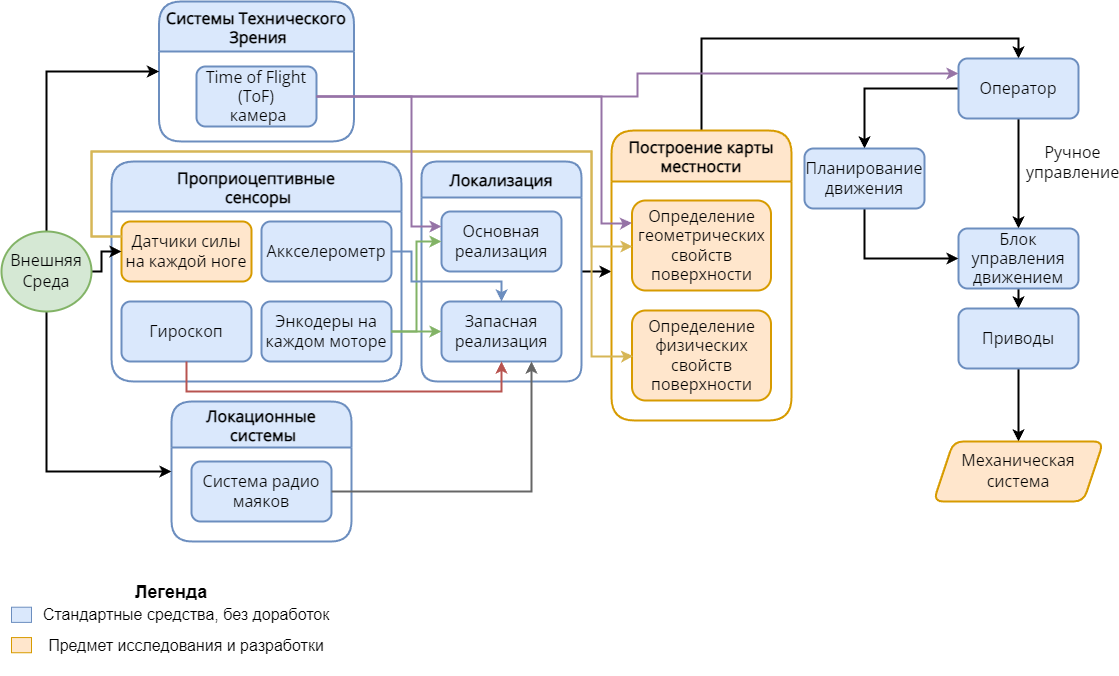
\includegraphics[width=0.9\textwidth,keepaspectratio]{main_diag_hor.png}
    \caption{Структурная схема разработанной системы}
    \label{fig:diag_system.png}
\end{figure}